\chapter{Waves, Quanta, and the First Picture of a Quantum Field}

Quantum field theory is the tool of the trade, but the lecture begins by refusing to define it too quickly. We first assemble the language of oscillations, then connect waves to photons and matter quanta, then make space finite in a way that preserves momentum, and only after that return to the harmonic oscillator and its operator language. These notes follow Leonard Susskind's lecture order closely, with curation by LazyingArt LLC, so that the mathematics arrives for the same reasons it arrives on the blackboard.

\section{Waves as the First Field Language}

A field is something that varies throughout space. A wave is a moving field configuration. Since waves are the simplest visible examples of fields, the lecture begins by reviewing the mathematics of oscillation rather than by defining quantum field theory outright.

The hallmark of an exponential is that its rate of change is proportional to the function itself:
\begin{equation}
\frac{d}{dx}e^{\alpha x}=\alpha e^{\alpha x}.
\end{equation}
That is the compact way to say that each small step in \(x\) changes the function by an amount proportional to what is already there.

Sines and cosines behave differently. They do not reproduce themselves under differentiation; instead they rotate into one another:
\begin{align}
\frac{d}{dx}\sin(kx)&=k\cos(kx),\\
\frac{d}{dx}\cos(kx)&=-k\sin(kx).
\end{align}
Because of this pair of relations, the combination \(\cos(kx)+i\sin(kx)\) behaves like an exponential of an imaginary quantity:
\begin{equation}
e^{ikx}=\cos(kx)+i\sin(kx),
\end{equation}
and differentiating it returns
\begin{equation}
\frac{d}{dx}e^{ikx}=ik\,e^{ikx}.
\end{equation}

This is the first useful piece of wave language. If \(x\) is a spatial coordinate, the same formulas describe oscillation in space. If \(x\) is time, they describe oscillation in time. The lecture keeps this point in reserve because frequency, wavelength, and later the Schr\"odinger equation will all be written in exactly this compact language.

\section{Wave Kinematics and Photon Energy-Momentum}

Now we put the ordinary wave bookkeeping on the board. The frequency \(f\) counts cycles per second, the angular frequency \(\omega\) counts radians per second, and \(\lambda\) denotes wavelength. For light we have the familiar relation
\begin{align}
\omega &= 2\pi f,\\
\lambda f &= c,\\
\frac{f}{c} &= \frac{1}{\lambda}.
\end{align}
The last two equations are not pure definitions; they say that the wave moves at the speed of light.

\begin{figure}[t]
\centering

\includegraphics[width=0.78\textwidth]{lecture_02_figure_03.png}
\caption{Two-column board of wave and momentum formulas.}
\end{figure}

Quantum mechanics enters through Planck's constant. The old notation is \(h\), the newer and more economical notation is
\begin{equation}
\hbar=\frac{h}{2\pi}.
\end{equation}
For one quantum of a wave, the energy is
\begin{equation}
E=\hbar\omega=hf.
\end{equation}
This is not the energy of an entire classical electromagnetic wave; it is the energy of one photon associated with that wave.

The lecture then turns immediately to momentum, because energy and momentum are the good bookkeeping devices of particle physics. For a nonrelativistic particle one writes
\begin{equation}
\vec p = m\vec v,
\end{equation}
but a photon has zero rest mass, so that is not the right formula for light. For a collimated light beam, or for one photon within it, the magnitude of the momentum is
\begin{equation}
|p|=\frac{E}{c}.
\end{equation}
Combining this with the wave relations gives the first real payoff of the lecture:
\begin{align}
|p_{\text{photon}}|
   &= \frac{E}{c}
    = \frac{hf}{c}
    = h\frac{f}{c}
    = \frac{h}{\lambda}.
\end{align}

\begin{figure}[t]
\centering

\includegraphics[width=0.54\textwidth]{lecture_02_figure_02.png}
\caption{Wave relations used in the photon-momentum step.}
\end{figure}

The point is not merely that we have derived a formula. The point is the physical moral attached to it: if we want short wavelength in order to probe small distances, then we must pay with large momentum. This is one of the main reasons high-energy particle physics is the way it is.

\subsection{Question \& Answer}
\paragraph{Where does \(E=\hbar\omega\) come from?}
The lecture does not derive that formula at this moment. Susskind answers the question by sending us back to the quantum mechanics of the harmonic oscillator. That is the deeper source of the relation, and later in the lecture we come back to the harmonic oscillator precisely because it is the mechanism behind this formula.

\subsection{Question \& Answer}
\paragraph{What does the amplitude of a wave mean once we speak in photons?}
A classical wave has more data than frequency and wavelength alone. It also has amplitude. If we compare two waves with the same wavelength and the same frequency, but with one much taller than the other, then what has changed is not the oscillation rate but the size of the field excursion.

\begin{figure}[t]
\centering
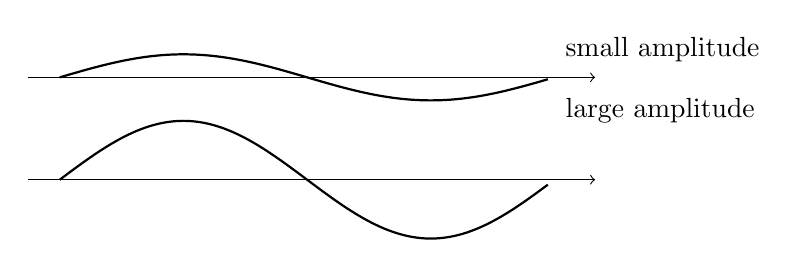
\begin{tikzpicture}[x=1cm,y=0.65cm]
\draw[->] (-0.4,0) -- (6.8,0);
\draw[->] (-0.4,-2.0) -- (6.8,-2.0);
\draw[thick] plot[domain=0:6.2,samples=120] (\x,{0.45*sin(\x r)});
\draw[thick] plot[domain=0:6.2,samples=120] (\x,{-2+1.15*sin(\x r)});
\draw (6.3,0.55) node[right]{small amplitude};
\draw (6.3,-0.65) node[right]{large amplitude};
\end{tikzpicture}
\caption{Two waves with the same frequency and wavelength but different amplitudes.}
\end{figure}

For the lecture the essential statement is only an order-of-magnitude one. Classically, the energy carried by the wave is proportional to the square of the amplitude,
\begin{equation}
E_{\text{wave}}\propto A^2.
\end{equation}
Quantum mechanically, if the wave consists of \(n\) photons of one frequency \(\omega\), then
\begin{equation}
E_{\text{wave}} = n\hbar\omega.
\end{equation}
Therefore, at fixed frequency,
\begin{equation}
A^2 \propto n\hbar\omega,
\qquad
A \propto \sqrt{n}.
\end{equation}

This should be kept in exactly that cautious form. The lecture does not work out normalization constants. It also insists that the question is partly ambiguous: amplitude and phase are not simultaneously sharp quantum observables. So for one photon we should read this only as an order-of-magnitude statement, obtained by setting \(n=1\).

A useful correction is also made here. In the standard picture of an electromagnetic wave moving along the \(x\)-axis, the vertical direction in the sine-wave sketch is not another spatial axis along which the photon wanders. It is the value of the electric or magnetic field. Only one axis in that picture is the direction of propagation.

\section{Which Relations Are General? Slow Matter Waves and Their Velocities}

Having used the light-wave formulas, the lecture stops and sorts them by generality. Definitions such as \(f\), \(\omega=2\pi f\), and \(\lambda\) are harmless. The relation \(E=\hbar\omega=hf\) is broad in scope. But anything with an explicit \(c\) in it should be treated cautiously: it is special to waves whose propagation speed is the speed of light. What survives as the general relation is
\begin{equation}
p=\frac{h}{\lambda}.
\end{equation}

\begin{figure}[t]
\centering

\includegraphics[width=0.72\textwidth]{lecture_02_figure_04.png}
\caption{Photon momentum written as \(hf/c=h/\lambda\).}
\end{figure}

This is the point at which the lecture turns from photons to matter waves. Electrons also diffract and interfere, so they too carry wavelength. Let us write their wave as \(\psi\). The question is no longer what the momentum is; that part is already fixed by \(p=h/\lambda\). The question is what relation between frequency and wavelength replaces \(\lambda f=c\) for a slowly moving particle.

For a nonrelativistic particle,
\begin{equation}
E=\frac{1}{2}mv^2=\frac{p^2}{2m}.
\end{equation}
Now combine this with the wave-particle dictionary:
\begin{align}
E &= hf,\\
p &= \frac{h}{\lambda}.
\end{align}
Then
\begin{align}
hf &= \frac{p^2}{2m}
   = \frac{1}{2m}\left(\frac{h}{\lambda}\right)^2,
\end{align}
and dividing by \(h\) gives
\begin{equation}
f=\frac{h}{2m\lambda^2}.
\end{equation}

\begin{figure}[t]
\centering

\includegraphics[width=0.62\textwidth]{lecture_02_figure_05.png}
\caption{Nonrelativistic energy and matter-wave frequency relation.}
\end{figure}

This is the crucial contrast. For light, frequency scales like \(1/\lambda\). For a slow particle, frequency scales like \(1/\lambda^2\). The lecture explicitly tells us not to memorize the formula as an isolated fact. One can always rederive it from two ingredients: the energy-momentum relation appropriate to the regime and the general relation \(p=h/\lambda\).

\subsection{Question \& Answer}
\paragraph{Which velocity of a matter wave packet should be identified with the particle?}
If we take a single monochromatic component of wavelength \(\lambda\), its phase velocity is
\begin{equation}
v_{\phi}=f\lambda=\frac{h}{2m\lambda}.
\end{equation}
Because this depends on \(\lambda\), different wavelengths propagate with different phase velocities. That means a localized wave packet cannot move as though all of its parts were locked together.

\begin{figure}[t]
\centering
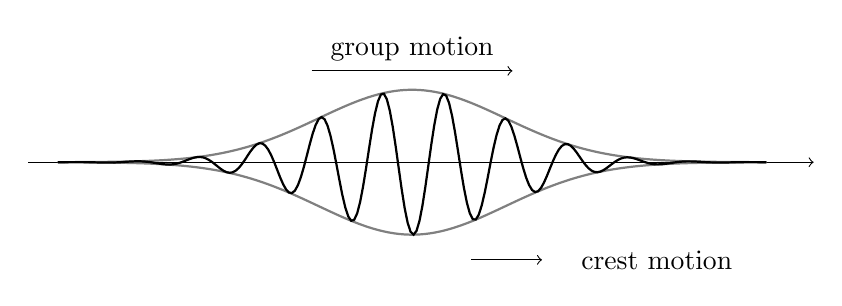
\begin{tikzpicture}[x=0.75cm,y=0.8cm]
\draw[->] (-0.5,0) -- (12.8,0);
\draw[thick,gray] plot[domain=0:12,samples=140] (\x,{1.15*exp(-0.20*(\x-6)^2)});
\draw[thick,gray] plot[domain=0:12,samples=140] (\x,{-1.15*exp(-0.20*(\x-6)^2)});
\draw[thick] plot[domain=0:12,samples=240] (\x,{1.15*exp(-0.20*(\x-6)^2)*sin(6*\x r)});
\draw[->] (4.3,1.45) -- (7.7,1.45);
\draw (6.0,1.8) node{group motion};
\draw[->] (7.0,-1.55) -- (8.2,-1.55);
\draw (8.7,-1.55) node[right]{crest motion};
\end{tikzpicture}
\caption{A schematic wave packet: the envelope and the interior crests generally move with different velocities.}
\end{figure}

The lecture therefore distinguishes two velocities. The phase velocity is the motion of the crests and troughs. The group velocity is the motion of the packet as a whole. The particle is identified with the group velocity, not the phase velocity.

This is also the place where the lecture makes a sharp conceptual remark: the nonrelativistic relation between frequency and wavelength is really the Schr\"odinger equation in condensed form. Frequency encodes time dependence; wavelength encodes spatial dependence. The Schr\"odinger equation is precisely the relation between those two dependences.

There is also a special case. If all wavelengths move with the same speed, then the packet and the internal crests move together. That is what happens for light in vacuum. There the phase velocity and the group velocity coincide. For dispersive matter waves they do not. The lecture even remarks that the phase velocity can exceed the speed of light, but that carries no signal and no contradiction, because information travels with the group velocity.

\section{Finite Space, Periodic Space, and Quantized Momentum}

The next shift in the lecture is methodological. Ultimately we care about waves in infinite space, but we do not begin there. Computers do not like infinity, and more to the point, the physics becomes cleaner if we first formulate the problem in a finite setting and only later take the large-volume limit.

So let us reduce space to one dimension. One possibility is an interval of length \(L\) with reflecting ends, like a violin string fixed at both ends. A wave then travels, reaches the boundary, reflects, and travels back. This is perfectly legitimate physics, but it has an immediate drawback: the momentum changes sign at reflection.

\subsection{Question \& Answer}
\paragraph{How do we make space finite without destroying momentum conservation?}
The lecture's answer is to identify the two ends of the interval. One should not imagine an ordinary geometric circle too literally; the point is only that the space is periodic. When a wave reaches one end, it reappears at the other and keeps moving in the same direction. Nothing special happens at the identification point, so momentum need not flip.

\begin{figure}[t]
\centering

\includegraphics[width=0.70\textwidth]{lecture_02_figure_06.png}
\caption{Schematic path of total length \(L\).}
\end{figure}

\begin{figure}[t]
\centering
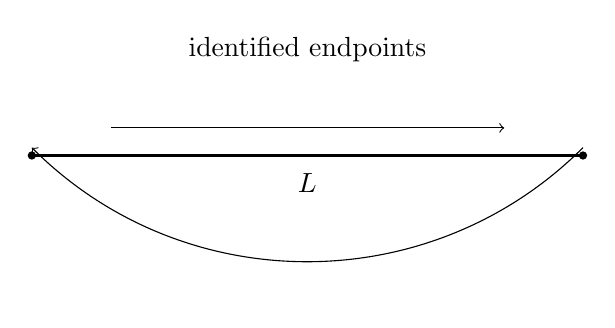
\begin{tikzpicture}[x=1cm,y=1cm]
\draw[thick] (0,0) -- (7,0);
\fill (0,0) circle (1.5pt);
\fill (7,0) circle (1.5pt);
\draw[->] (1.0,0.35) -- (6.0,0.35);
\draw (3.5,-0.35) node{\(L\)};
\draw[->,bend left=45] (7,0.1) to (0,0.1);
\draw (3.5,1.35) node{identified endpoints};
\end{tikzpicture}
\caption{A cleaned reconstruction of the periodic identification. The geometry is schematic: the point is periodicity, not an embedded circle.}
\end{figure}

Once space is periodic, wavelengths become discrete. An integer number of wavelengths must fit around the total length \(L\), so
\begin{equation}
\lambda_N=\frac{L}{N},
\qquad
N=1,2,3,\dots
\end{equation}
and therefore the allowed momenta are also discrete:
\begin{equation}
p_N=\frac{h}{\lambda_N}=\frac{Nh}{L}.
\end{equation}
Momentum is quantized not because we have added a mysterious extra rule, but because periodicity only allows certain wavelengths.

A wave packet causes no difficulty here. It is simply a superposition of allowed plane waves. In other words, Fourier analysis still works, but the allowed Fourier modes are now discrete rather than continuous.

The lecture then briefly reformulates the same result for a genuine circular wire of radius \(r\), with circumference \(L=2\pi r\). In that case
\begin{equation}
p_n=\frac{nh}{2\pi r}.
\end{equation}
Multiplying by \(r\) turns this into angular momentum quantization:
\begin{equation}
J = rp_n = n\hbar.
\end{equation}
Here it is cleaner to write \(J\) for angular momentum, since the lecture momentarily lets the symbol \(L\) collide with two different meanings.

\section{Quantum-Mechanical Machinery: Commutators and One Harmonic Oscillator}

After the break the lecture finally turns to the piece of quantum mechanics it needs in order to say what a quantum field is. The first notion is the commutator. For two operators \(A\) and \(B\),
\begin{equation}
[A,B]=AB-BA.
\end{equation}
If this vanishes, the lecture interprets that as the statement that the two corresponding observables can be measured simultaneously. If it does not vanish, measuring one interferes with measuring the other. The order of operations matters.

For the ordinary particle variables, the lecture recalls the basic pattern. The components of position commute with one another. The components of momentum commute with one another. But a position component and the corresponding momentum component do not:
\begin{equation}
[x,p_x]=i\hbar.
\end{equation}
Likewise for \(y\) with \(p_y\), and \(z\) with \(p_z\). By contrast, mixed components such as \(x\) and \(p_y\) can be measured together.

The real target, however, is the harmonic oscillator. Waves oscillate, so the harmonic oscillator is the elementary quantum system from which the field description will be built. The lecture adopts the convenient convention that the lowest energy is shifted to zero. With that convention, the allowed energies are
\begin{equation}
E_n = n\hbar\omega,
\qquad
n=0,1,2,\dots
\end{equation}
and the state with energy \(E_n\) is denoted by the ket \(|n\rangle\).

\begin{figure}[t]
\centering
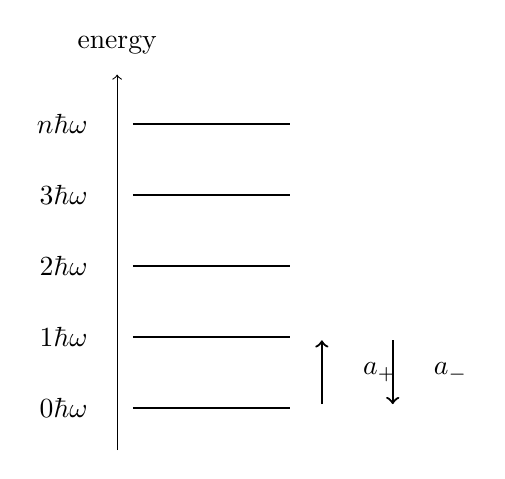
\begin{tikzpicture}[x=1cm,y=0.9cm]
\draw[->] (0,0) -- (0,5.3);
\draw (0,5.45) node[above]{energy};
\foreach \y/\n in {0.6/0,1.6/1,2.6/2,3.6/3,4.6/n}
{
  \draw[thick] (0.2,\y) -- (2.2,\y);
  \draw (-0.25,\y) node[left]{\(\n\hbar\omega\)};
}
\draw[->,thick] (2.6,0.65) -- (2.6,1.55);
\draw (3.0,1.1) node[right]{\(a_+\)};
\draw[->,thick] (3.5,1.55) -- (3.5,0.65);
\draw (3.9,1.1) node[right]{\(a_-\)};
\end{tikzpicture}
\caption{A cleaned energy-level picture of the shifted harmonic oscillator.}
\end{figure}

Now come the raising and lowering operators, written in the lecture as \(A+\) and \(A-\), and here rendered as \(a_+\) and \(a_-\) to stay close to that notation:
\begin{align}
a_+|n\rangle &= \sqrt{n+1}\,|n+1\rangle,\\
a_-|n\rangle &= \sqrt{n}\,|n-1\rangle,\\
a_-|0\rangle &= 0.
\end{align}
These are not classical observables in the ordinary sense. They are operations that move us up and down the tower of oscillator states, adding or removing one quantum of energy of fixed frequency \(\omega\).

A short piece of algebra already shows why order matters. Acting first with \(a_-\) and then with \(a_+\) gives
\begin{equation}
a_+a_-|n\rangle = n|n\rangle,
\end{equation}
while the opposite order gives
\begin{equation}
a_-a_+|n\rangle = (n+1)|n\rangle.
\end{equation}
So the two orders differ by one unit. In that sense these operators are genuinely quantum-mechanical objects: they do not commute, and their noncommutativity is tied to the impossibility of making the corresponding amplitude-and-phase information simultaneously sharp.

If the oscillator is an electromagnetic mode, these same operators become creation and annihilation operators for photons. They add and remove quanta of the field.

\section{From Many Oscillators to a Quantum Field}

We can now return to the periodic world of length \(L\). Once the allowed wavelengths are discrete,
\begin{equation}
\lambda_N=\frac{L}{N},
\end{equation}
the allowed frequencies are also discrete. Let us call them \(\omega_N\). Each allowed mode \(N\) is one harmonic oscillator. A field is therefore not one oscillator but an entire collection of them, one for each allowed frequency.

For each mode \(N\), we may have \(n_N\) quanta. The natural state label is then
\begin{equation}
|n_1,n_2,n_3,\dots\rangle.
\end{equation}
This is the point at which the lecture has to disentangle two different integers. One integer labels the mode: that is \(N\), the number that tells us which wavelength or frequency we are talking about. The other integer labels the occupation of that mode: that is \(n_N\), the number of quanta placed in that oscillator.

If we think of a violin string, the analogy becomes vivid. The fundamental mode has its own frequency. The first harmonic has a higher frequency. The next harmonic is higher still. Each one is its own oscillator, and each one can carry zero, one, two, or many quanta. The whole state of the string is specified only after we say how much quantized energy sits in every mode.

In this elementary setting the field energy is therefore built mode by mode:
\begin{equation}
E=\sum_{N} n_N \hbar \omega_N.
\end{equation}
Likewise there is a creation operator and an annihilation operator for each mode. That is the mathematical content of the lecture's claim that a quantum field is a collection of harmonic oscillators.

This is also why the operator language matters for particle physics. In an experiment, particles with given energies and momenta come in, and particles with other energies and momenta go out. The formalism must therefore know how to remove quanta from an initial state and add quanta to a final state. That is exactly what annihilation and creation operators do. They are not decorative notation; they are the language in which particle processes are written.

\section{Summary}

The lecture begins by postponing the definition of quantum field theory and backing up to the wave mathematics it will need. From exponentials, sines, and cosines we pass to frequency and wavelength, from there to photon energy and momentum, and from there to the more general relation \(p=h/\lambda\). Slow matter waves then force us to distinguish light-specific formulas from general ones and to separate phase velocity from group velocity. Periodic space discretizes momentum, and after the break the harmonic oscillator provides the missing quantum-mechanical machinery. The chapter therefore ends where the lecture means to end: a quantum field is an infinite collection of oscillators, one for each mode, together with operators that add and subtract quanta in those modes.